\documentclass{beamer}

\usepackage[frenchb]{babel}
\usepackage[T1]{fontenc}
\usepackage[utf8]{inputenc}

\usetheme{Warsaw}


\begin{document}

	\begin{frame}
	\frametitle{Projet de C++}
	\framesubtitle{Le voyageur de commerce}
		\begin{center}
			Soutenance de projet\\
			05/05/2017\\
			CARON Alexandre, COLLOT Kévin, LEMAN Jean-Christophe
		\end{center}	
	\end{frame}

	\begin{frame}
	\frametitle{Projet de C++}
	\framesubtitle{Introduction}
		\textbf{Objectifs:}
		\begin{itemize}
		\item Résolution du problème du voyageur de commerce
		\item Utilisation d'un algorithme génétique
		\end{itemize}
	\end{frame}

	\begin{frame}
	\frametitle{Projet de C++}
	\framesubtitle{Présentation du groupe}
		\textbf{Rôles:}	
		\begin{itemize}
		\item CARON Alexandre: Mutations, sélections.
		\item COLLOT Kévin: Interface graphique.
		\item LEMAN Jean-Christophe: Algorithme principal.
		\end{itemize}
	\end{frame}
	
	\begin{frame}
	\frametitle{Projet C++}
	\framesubtitle{Manuel utilisateur}
		\textbf{Se placer dans le répertoire "class" puis utiliser le makefile qui se charge de:}
		\begin{itemize}
		\item Compiler la bibliothèque CNG,
		\item Créer tous les objets,
		\item Créer le fichier main.exe à exécuter.
		\end{itemize}
	\end{frame}

	\begin{frame}
	\frametitle{Projet C++}
	\framesubtitle{Difficultés rencontrées}	
		\begin{itemize}
		\item Compréhension de la notion d'algorithme génétique,
		\item Gestions des nombreuses classes nécessaires,
		\item Implantation du code.
		\end{itemize}
	\end{frame}
	
	\begin{frame}
	\frametitle{Projet C++}
	\framesubtitle{Perspectives d'évolution}
		\begin{itemize}
		\item Ajout d'autres méthodes de sélections,
		\item Ajout de nouvelles possibilités d'interaction entre l'interface et l'utilisateur,
		\item Améliorer la vitesse d'exécution. 
		\end{itemize}			
	\end{frame}
	
	\begin{frame}
	\frametitle{Projet C++}
	\framesubtitle{Quelques résultats}
	
	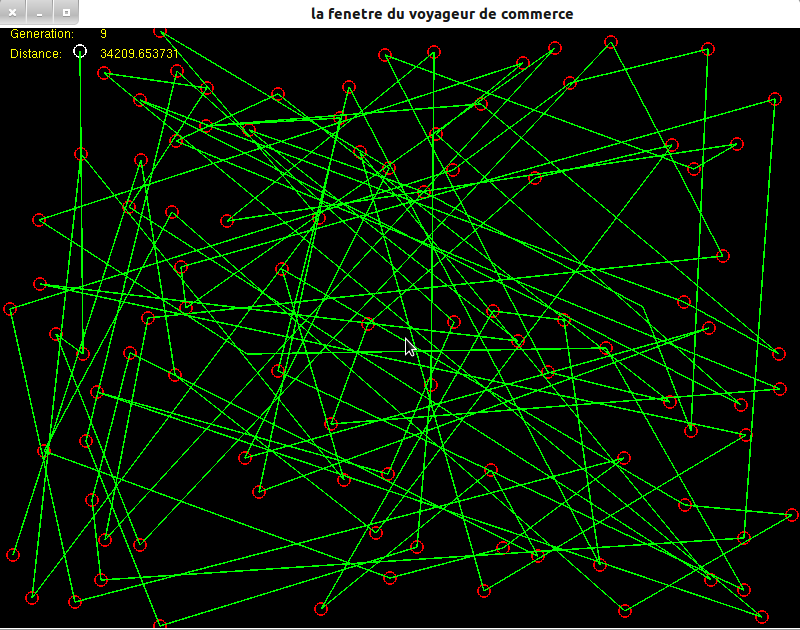
\includegraphics[scale=0.2]{1.png}
	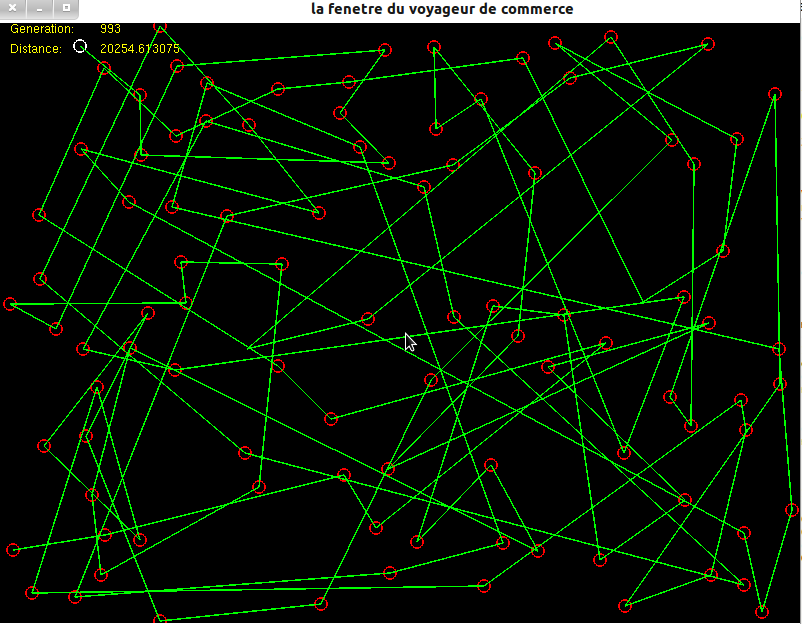
\includegraphics[scale=0.2]{2.png}
			
	\end{frame}
	
	\begin{frame}
	\frametitle{Projet C++}
	\framesubtitle{Quelques résultats}
	
	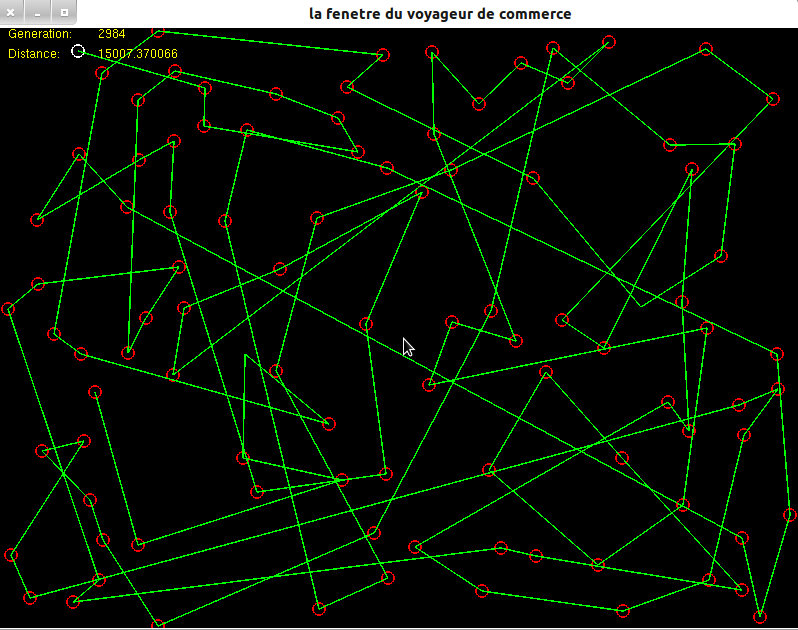
\includegraphics[scale=0.2]{3.png}
	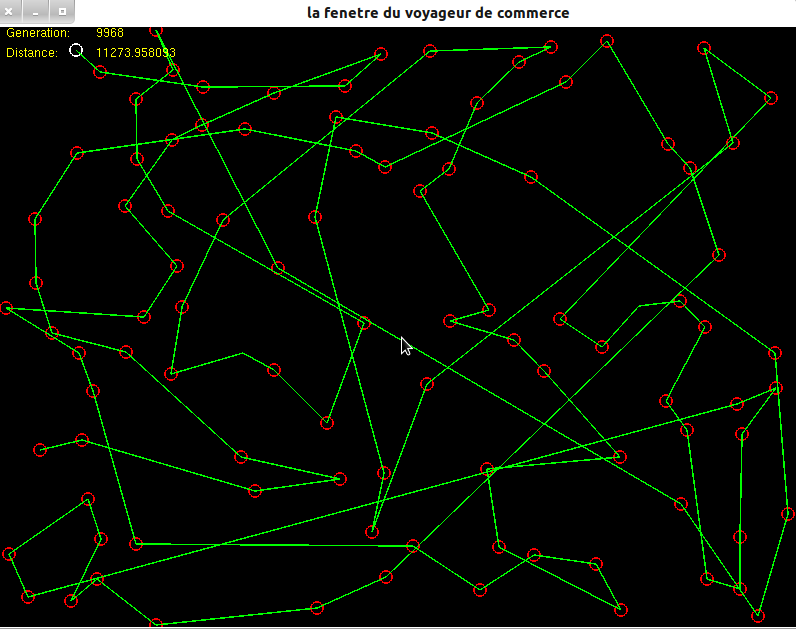
\includegraphics[scale=0.2]{4.png}
			
	\end{frame}		
	
	\begin{frame}
	\frametitle{Projet C++}
	\framesubtitle{Quelques résultats}
	
	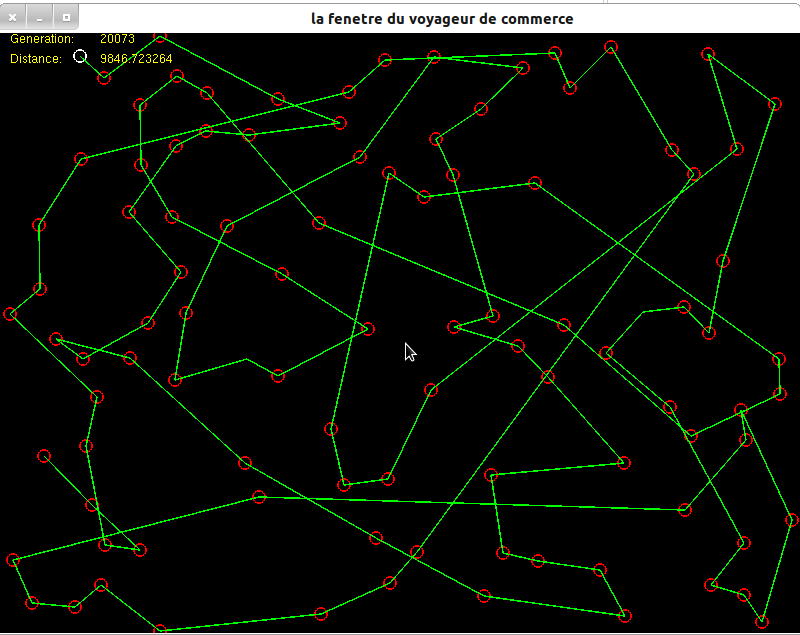
\includegraphics[scale=0.2]{5.png}
	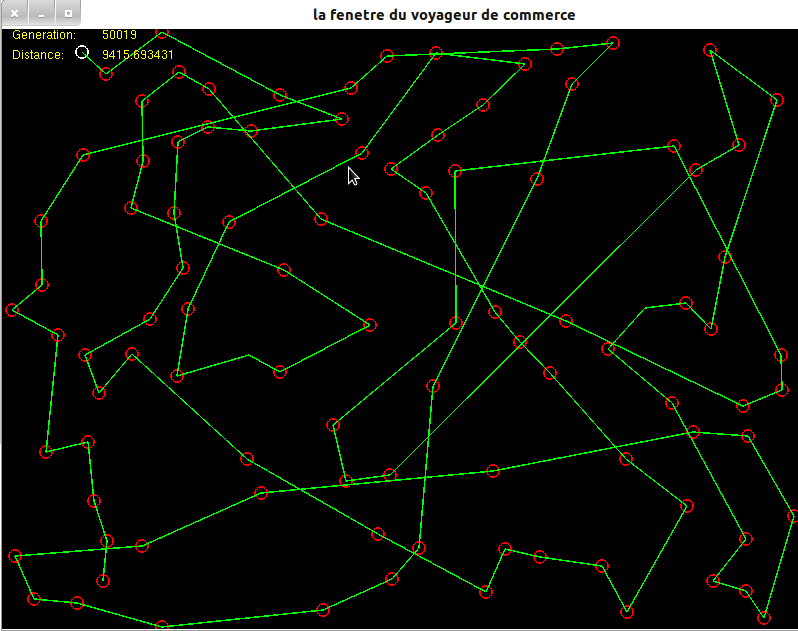
\includegraphics[scale=0.2]{6.png}
			
	\end{frame}		
	
\end{document}